\documentclass{standalone}
\usepackage{pgfplots}
\usepackage{amsmath}
\newcommand{\textbox}[2]{\setbox0=\hbox{$#2$}\typeout{BOX #1: \the\wd0,\the\ht0,\the\dp0}}
\newcommand{\point}[2]{\pgfextractx{\dimen0}{\pgfpointanchor{#1}{#2}}\pgfextracty{\dimen2}{\pgfpointanchor{#1}{#2}}\typeout{POINT #1.#2: \the\dimen0,\the\dimen2}}
\begin{document}
\textbox{cos}{\cos x}
\textbox{x}{x}
\textbox{fraction}{\varphi_1(x)=\frac{1}{1+e^{-x}}}
\textbox{max}{\varphi_5(x)=\max(x,e^x-1)}
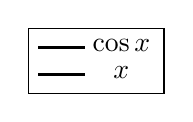
\begin{tikzpicture}
\matrix[/pgfplots/every axis legend,fill=none,at={(0,0)},anchor=north] (L) {
\draw[very thick] plot coordinates {(0,0)(.3,0)(.6,0)}; \coordinate (S1) at (0,0); & \node (T1) {$\cos x$};\\
\draw[very thick] plot coordinates {(0,0)(.3,0)(.6,0)}; \coordinate (S2) at (0,0); & \node (T2) {$x$};\\
};
\point{L}{north west}\point{L}{south east}
\point{T1}{center}\point{T1}{text}\point{T1}{west}\point{T1}{north}\point{T1}{south}
\point{T2}{center}\point{T2}{text}\point{T2}{north}\point{T2}{south}
\point{S1}{center}\point{S2}{center}
\end{tikzpicture}
{\tiny\textbox{tiny-matrix}{\begin{pmatrix}0\\-42\end{pmatrix}+U}}
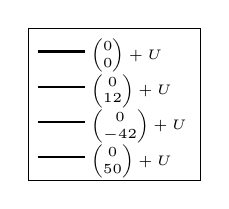
\begin{tikzpicture}
\matrix[/pgfplots/every axis legend,font=\tiny,cells={anchor=west},at={(0,0)},anchor=north west] (L) {
\draw[thick] plot coordinates {(0,0)(.3,0)(.6,0)}; \coordinate (S1) at (0,0); & \node (T1) {$\begin{pmatrix}0\\0\end{pmatrix}+U$};\\
\draw[thick] plot coordinates {(0,0)(.3,0)(.6,0)}; \coordinate (S2) at (0,0); & \node (T2) {$\begin{pmatrix}0\\12\end{pmatrix}+U$};\\
\draw[thick] plot coordinates {(0,0)(.3,0)(.6,0)}; & \node {$\begin{pmatrix}0\\-42\end{pmatrix}+U$};\\
\draw[thick] plot coordinates {(0,0)(.3,0)(.6,0)}; & \node {$\begin{pmatrix}0\\50\end{pmatrix}+U$};\\
};
\point{L}{north west}\point{L}{south east}\point{T1}{center}\point{T1}{text}\point{T2}{text}
\point{S1}{center}\point{S2}{center}
\end{tikzpicture}
\end{document}
